%-----------------------------------------------------------------------------------------------------
\chapter{Results}
\label{cap:resultados_obtidos}
%-----------------------------------------------------------------------------------------------------

%-----------------------------------------------------------------------------------------------------
\section{Introduction}
%-----------------------------------------------------------------------------------------------------

This chapter presents the experimental results obtained from the characterisation of the antennas, the balun, the impedance matching PCB, and the 868~MHz band-pass filter, as well as from the complete antenna radiation pattern measurement system. The band-pass filter, based on SAW (Surface Acoustic Wave) technology, was included in the setup to suppress out-of-band noise and interference. The initial objective of these measurements was to validate the performance of the antennas individually, both the transmitting and receiving antennas, which exhibit very similar, though not identical, behaviour due to slight manufacturing differences.

Measurements were carried out mainly with a VNA, supported by an RF signal generator and, in some cases, with a Spectrum Analyzer (SA). For each element, $S_{11}$ and, where relevant, $S_{21}$ parameters were measured to evaluate impedance matching, signal integrity, and the suppression of undesired common modes. All measurements are presented together with their corresponding plots for clarity.

Among the different characterisations, the antenna radiation pattern was of particular interest, as it directly reflects the Yagi-Uda design and provides a key indicator of the overall system performance.


%-----------------------------------------------------------------------------------------------------
\section{Measurement Setup}
%-----------------------------------------------------------------------------------------------------

The objective of this measurement setup was to obtain the horizontal (azimuth) radiation pattern of the antenna under test and to validate the far-field measurement conditions.

The transmitting and receiving antennas were initially characterised using a NanoVNA at 868~MHz. After that, the band-pass filter was also verified for compliance with the operating frequency requirements.

For the far-field radiation pattern measurement, the minimum far-field distance was calculated using (\ref{eq:farfield_distance}):

\begin{equation}
    d = \frac{2R^{2}}{\lambda}
    \label{eq:farfield_distance}
\end{equation}

where $R$ is the largest dimension of the antenna, equivalent to the boom length in the case of the Yagi-Uda, and $\lambda$ is the wavelength. For $R = 0.3~\text{m}$ and $\lambda \approx 0.345~\text{m}$, $d \approx 0.52~\text{m}$. To ensure far-field conditions, the antennas were spaced $D = 2.5~\text{m}$ apart.


The transmitting antenna was a Yagi-Uda with a gain of approximately $10~\text{dB}$, with a maximum input power of $0.5~\text{mW}$ ($-3~\text{dBm}$) to comply with an EIRP (Effective Isotropic Radiated Power) of 5~mW. Using the Friis equation (\ref{eq:friis}) \cite{Friis1946}, which relates transmitted and received power in free space, the expected received power can be calculated. Assuming an isotropic receiving antenna, the result is:

\begin{align}
    P_{\mathrm{rx}} &= P_{\mathrm{tx}} + G_{\mathrm{tx}} + G_{\mathrm{rx}} - 20 \log_{10} \left( \frac{4 \pi D}{\lambda} \right) \label{eq:friis} \\
    P_{\mathrm{rx}} &= -3 + 10 + 0 - 20 \log_{10} \left( \frac{4 \pi \times 2.5}{0.3456} \right)  \\
    P_{\mathrm{rx}} &\approx -32~\text{dBm (in free-space conditions).} 
\end{align}

Considering, however, that the receiving antenna is also a Yagi-Uda with a gain of about $10~\text{dB}$, the expected received power rises to approximately $-22$~dBm, which is in line with the measured results discussed later (between $-22$ and $-18$~dBm).

Measurements were performed outdoors to minimise multipath effects, with both antennas mounted at least 1~m above ground on fibreglass supports to reduce ground reflections. The receiving antenna was rotated in azimuth in $5^{\circ}$ steps, while the transmitting antenna remained fixed.

The signal power was measured using an AD8313 detector, calibrated before the measurements began. The calibration data were obtained from a reference measurement setup, as shown in Figure \ref{cap4:sec2:fig1}, and the relationship between the input signal power and the output voltage of the integrated circuit was determined using the weighted least squares method, as shown in:

\begin{equation}
    V_\text{out} = 0.0185 \cdot P_\text{in} + 1.8621
\end{equation}

yielding a sensitivity of approximately 19~mV/dBm, close to the 18~mV/dBm from the datasheet.

\begin{figure}[H]
    \centering
    % Left: larger image
    \begin{subfigure}{0.378\textwidth}
        \centering
        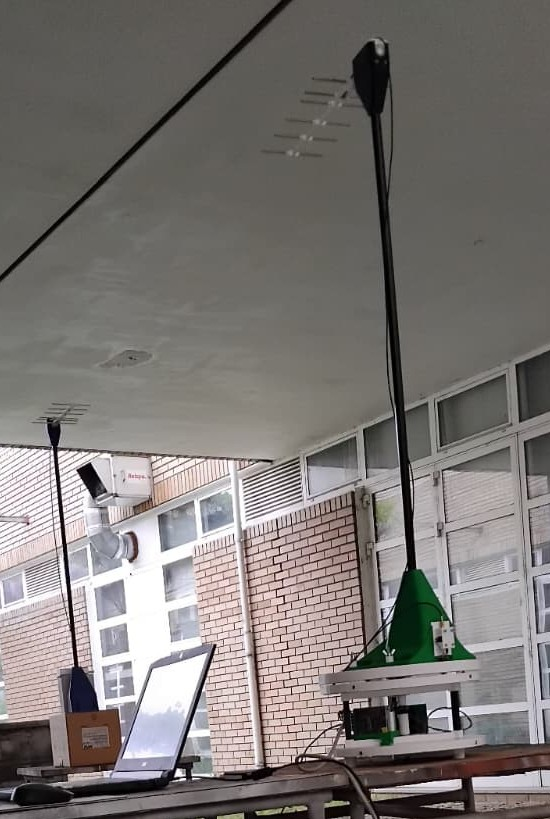
\includegraphics[width=\textwidth]{Imagens/setup1.jpg}
        \caption{Setup rear view}
        \label{fig:setup:a}
    \end{subfigure}
    \hspace{0.5mm}
    % Right: two smaller images stacked
    \begin{minipage}{0.6\textwidth}
        \begin{subfigure}{\textwidth}
            \centering
            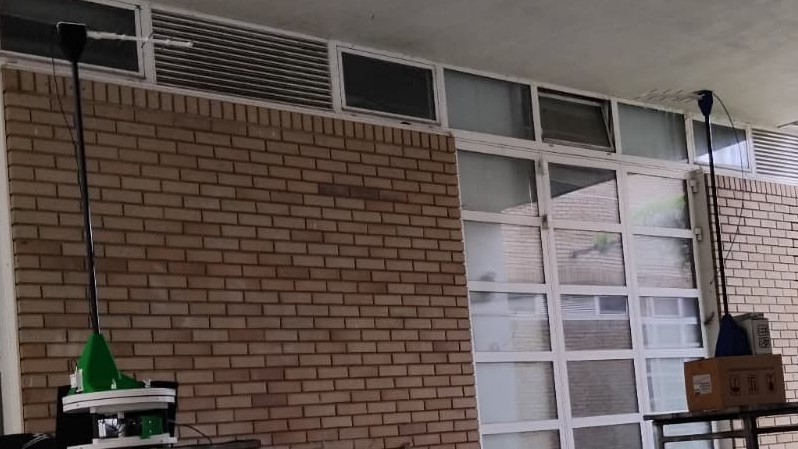
\includegraphics[width=0.76\textwidth]{Imagens/setup2.jpg}
            \caption{Setup side view(closer)}
            \label{fig:setup:b}
        \end{subfigure}
        \vskip 1mm
        \begin{subfigure}{\textwidth}
            \centering
            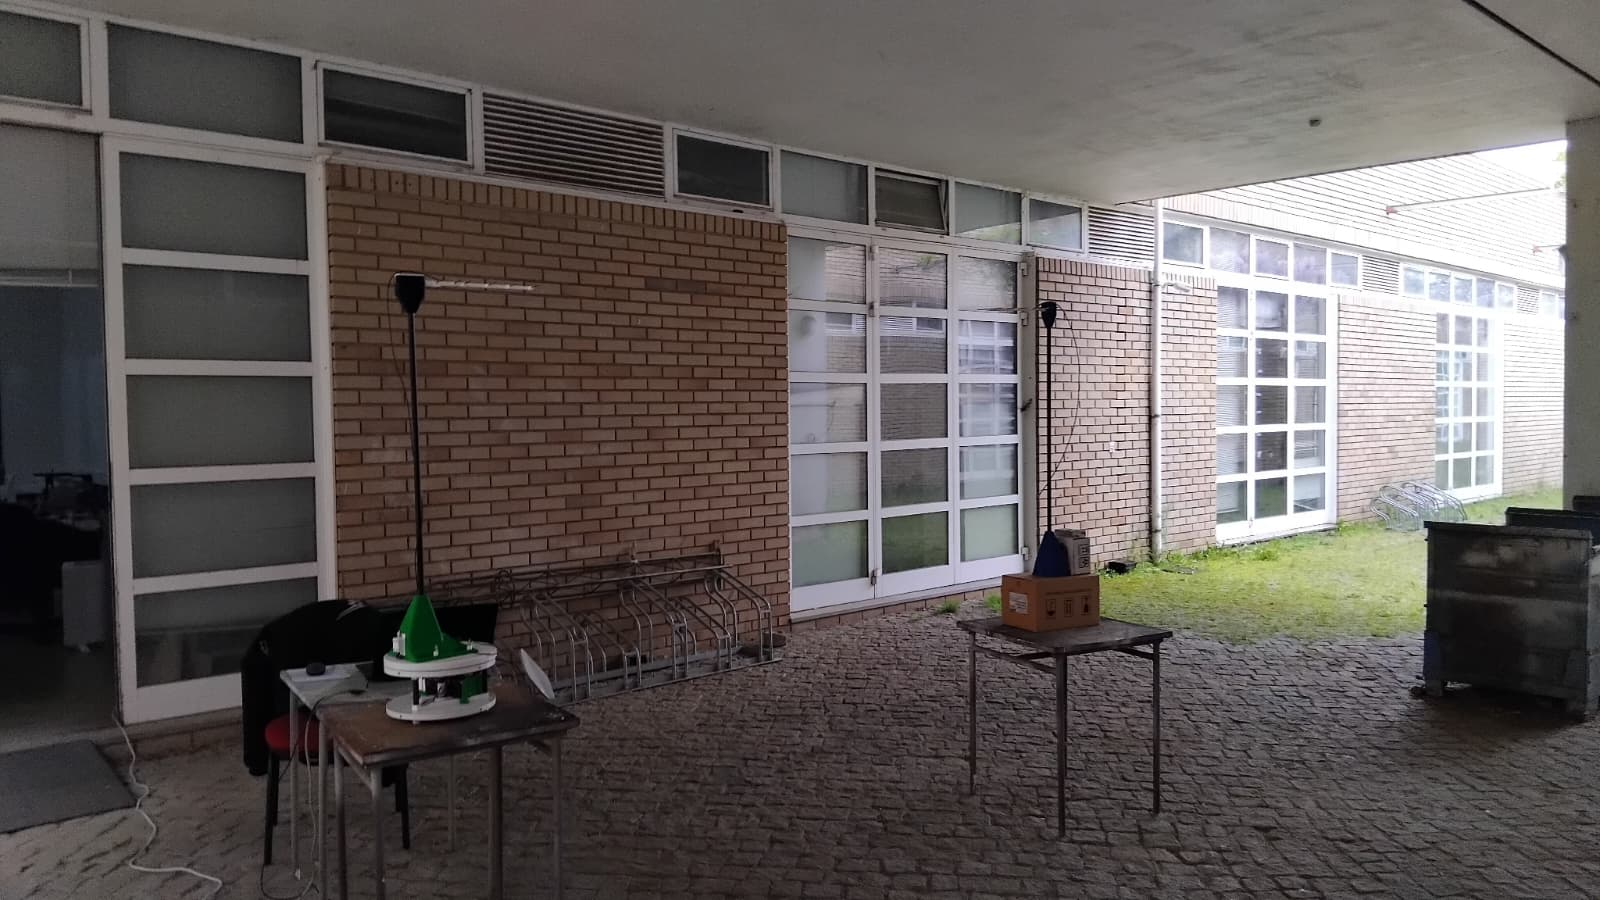
\includegraphics[width=0.76\textwidth]{Imagens/setup3.jpg}
            \caption{Setup side view}
            \label{fig:setup:c}
        \end{subfigure}
    \end{minipage}
    \caption{Experimental setup for transmitting and receiving antennas, showing rear and side perspectives.}
    \label{cap4:sec2:fig1}
\end{figure}


%-----------------------------------------------------------------------------------------------------
\section{Characterisation of Components}
%-----------------------------------------------------------------------------------------------------

The characterisation of the components was performed using the NanoVNAsaver\footnote{NanoVNAsaver is an open-source software that reads data from the NanoVNA and displays it on a computer.} and, where applicable, a TinySA (spectrum analyzer). Measurements focused on the relevant scattering parameters (S-parameters) of each component.

In this work, only the most relevant S-parameters are considered, namely $S_{11}$ and $S_{21}$. However, the others parameters are:

\begin{itemize}
    \item $S_{11}$: reflection coefficient at port 1, indicating the matching of the input impedance.

    \item $S_{21}$: forward transmission from port 1 to port 2, representing insertion loss or gain.

    \item $S_{22}$: reflection coefficient at port 2, indicating the matching of the output impedance.
    
    \item $S_{12}$: reverse transmission from port 2 to port 1, representing isolation or reverse gain.


\end{itemize}

In addition, to complement the analysis of impedance matching, the Voltage Standing Wave Ratio (VSWR) was also considered. VSWR is directly related to $S_{11}$ and indicates how effectively power is transferred from the source to the load, with values close to 1 indicating good matching, and values above 2 are generally considered poor.


%-----------------------------------------------------------------------------------------------------
\subsection{868~MHz Band-Pass Filter}
%-----------------------------------------------------------------------------------------------------

The measured response confirms that the filter effectively attenuates out-of-band signals and reduce unwanted noise, thereby improving the selectivity of the measurement system. Figure~\ref{cap4:sec3:subsec2:fig1} shows the measured $S_{21}$ parameter, representing the insertion loss.

\begin{figure}[H]
    \centering
    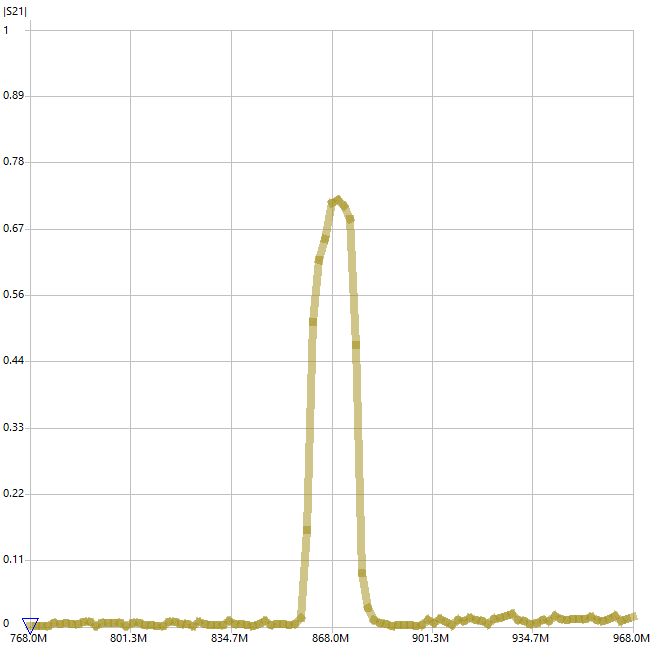
\includegraphics[width=0.72\textwidth]{Imagens/filtro/fig1.png}
    \label{cap4:sec3:subsec2:fig1:a}
    \caption{$S_{21}$ of the 868~MHz band-pass filter showing insertion loss and passband characteristics.}
    \label{cap4:sec3:subsec2:fig1}
\end{figure}

At the centre frequency of 868~MHz, the insertion loss is approximately 3~dB, which is consistent with the manufacturer’s specifications. The bandwidth extends from about 860~MHz to 880~MHz, typical of commercial ISM band-pass filters. This response ensures that the antenna operates effectively within the intended frequency range while suppressing frequencies outside it.


The measured attenuation will be taken into account in the subsequent radiation pattern measurements, as it directly affects the received signal strength.


%-----------------------------------------------------------------------------------------------------
\subsection{Balun}
%-----------------------------------------------------------------------------------------------------

The transmission coefficient $S_{21}$ of the balun was measured using a VNA to evaluate its performance in converting between balanced and unbalanced signals. The results, shown in Figure~\ref{cap4:sec3:subsec3:fig1}, indicate a differential mode insertion loss of approximately $-0.58$~dB at 868~MHz and a common mode attenuation greater than $-47$~dB at the same frequency. Additional measurements confirmed good impedance matching at both ports.
\vspace{-1em}
\begin{figure}[!ht]
    \centering
    \begin{subfigure}[b]{0.48\textwidth}
        \centering
        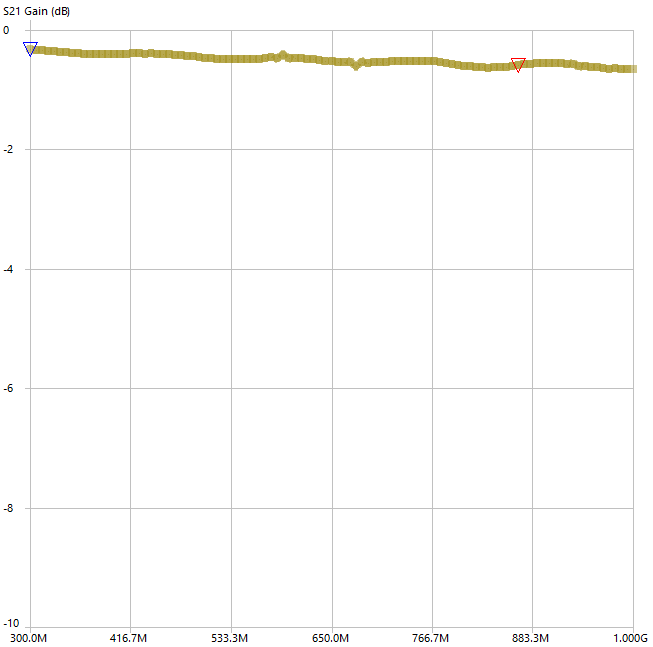
\includegraphics[width=\textwidth]{Imagens/balun_caract/insertion_loss.png}
        \caption{Differential mode: insertion loss of $\approx -0,58$~dB at 868~MHz.}
        \label{cap4:sec3:subsec3:fig1:a}
    \end{subfigure}
    \hfill
    \begin{subfigure}[b]{0.48\textwidth}
        \centering
        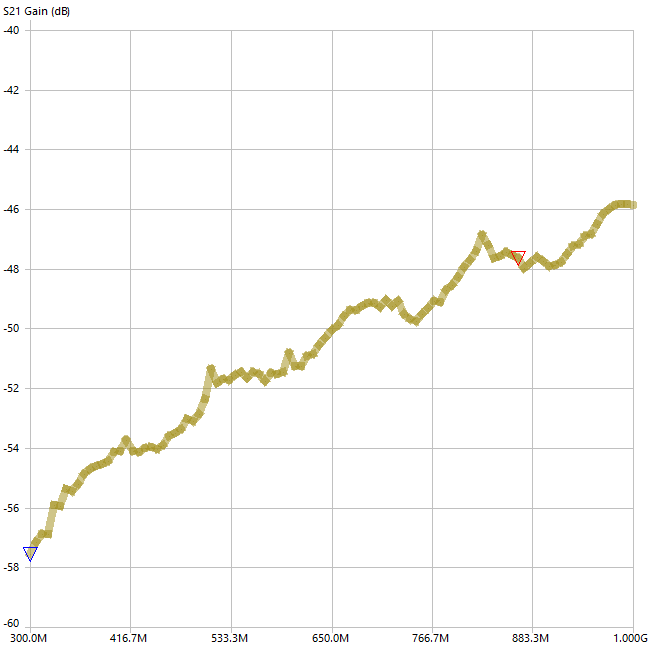
\includegraphics[width=\textwidth]{Imagens/balun_caract/insertion_loss2.png}
        \caption{Common mode: attenuation greater than $-47$ dB at 868 MHz.}
        \label{cap4:sec3:subsec3:fig1:b}
    \end{subfigure}
    \caption{Experimental S21 results for the air choke balun using VNA in differential and common modes.}
    \label{cap4:sec3:subsec3:fig1}
\end{figure}


%-----------------------------------------------------------------------------------------------------
\subsection{PCB for Impedance Matching}
%-----------------------------------------------------------------------------------------------------

The S-parameters of the PCB confirm the effectiveness of the impedance matching network, as shown in Figure \ref{cap4:sec3:subsec4:fig1}. 
At the 868~MHz frequency, the reflection coefficient at the input port is 
$S_{11} \approx -20.3$~dB. 
This translates to a VSWR of approximately $1.213$, close to the ideal value of~1. 
The input impedance measured at this frequency is $43.1 - j5.76~\Omega$, close to the nominal $50~\Omega$ reference. 
Such results demonstrate that the reflected power is reduced to below $1\%$, confirming an excellent matching performance. Other parameters were omitted, as they provided no further insight into the matching performance.

\begin{figure}[H]
    \centering
    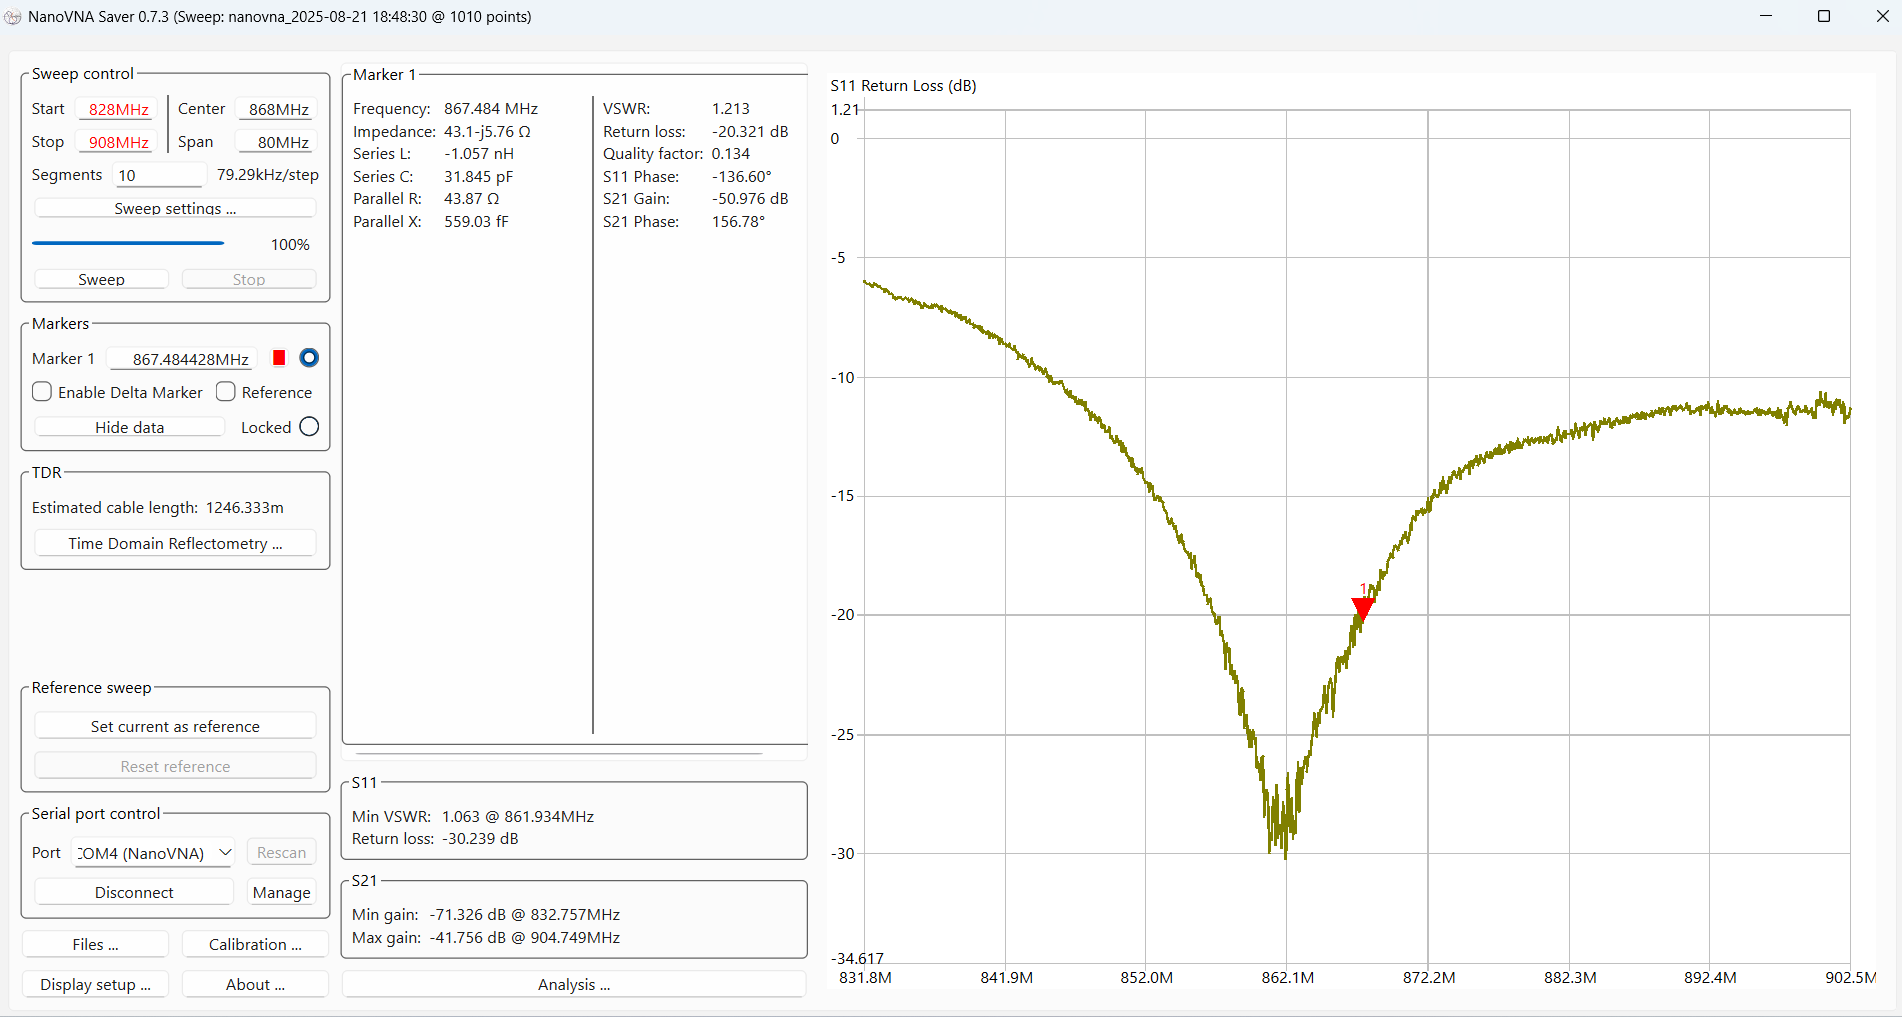
\includegraphics[width=0.98\textwidth]{Imagens/carcaterização do PCB/S11 e S21 v4 mais um L de 3.3 em serie complta Tx.png}
    \caption{$S_{11}$ graph and VSWR of the PCB used for impedance matching}
    \label{cap4:sec3:subsec4:fig1}
\end{figure}

%-----------------------------------------------------------------------------------------------------
\subsection{Reflection Coefficient and Matching Performance}
%-----------------------------------------------------------------------------------------------------

Matching improvement was quantified by evaluating the reflection coefficient ($\Gamma$) and reflected power. 
The relationships between return loss, reflection coefficient, and reflected power are well-established in microwave engineering \cite{pozar2011}.

The return loss (RL) is related to the voltage reflection coefficient $\Gamma$ as:
\begin{equation}
\label{eq:RL}
RL = -10 \log_{10}\left|\frac{P_{\text{refl}}}{P_{\text{inc}}}\right|
   = -20 \log_{10}\left|\frac{V_{\text{refl}}}{V_{\text{inc}}}\right|
   = -20 \log_{10}|\Gamma|
\end{equation}

Equivalently, the S-parameter $S_{11}$ is related to the reflection coefficient as:
\begin{equation}
\label{eq:S11}
S_{11} = -RL = 20 \log_{10} |\Gamma| \xrightarrow{} |\Gamma| = 10^{-\tfrac{RL}{20}}
\end{equation}

Finally, the fraction of reflected power can be expressed as:
\begin{equation}
\label{eq:Preflected}
P_{\text{refl}} = |\Gamma|^2
\end{equation}

These equations are directly related: the return loss determines the magnitude of the reflection coefficient, which in turn gives the fraction of reflected power. This allows an intuitive interpretation of matching performance in terms of the percentage of incident power that is reflected back. In practical terms, the complement $1-|\Gamma|^2$ corresponds to the fraction of power actually delivered to the load, providing a direct link between return loss and system efficiency. For instance, a return loss of 10~dB corresponds to about 10\% reflected power, while 20~dB corresponds to only 1\%, values that are typically regarded as acceptable or good in RF design.


\subsection*{Before Matching}
For a measured return loss of $RL \approx 11$~dB:
\begin{align}
|\Gamma| &= 10^{-\tfrac{RL}{20}} \label{eq:Gamma}\\
|\Gamma| &= 10^{-\tfrac{11}{20}} \approx 0.2818, \label{eq:GammaBefore}\\
P_{\text{refl}} &= (0.2818)^2 \approx 0.079 \ (\text{or } 7.9\%)
\end{align}

\subsection*{After Matching}
With the return loss improved to $RL \approx 20.3$~dB:
\begin{align}
|\Gamma| &= 10^{-\tfrac{RL}{20}} \\
|\Gamma| &= 10^{-\tfrac{20.3}{20}} \approx 0.096, \label{eq:GammaAfter}\\
P_{\text{refl}} &= (0.096)^2 \approx 0.0092 \ (\text{or } 0.92\%)
\end{align}

These results show that the reflected power was reduced from approximately 8\% to less than 1\% of the incident power, 
which corresponds to a significant improvement in power transfer efficiency. This analysis confirms that, despite the impedance of $43.1-j5.76 \ \Omega$, the antenna system exhibits significantly improved matching compared to the initial condition.
%-----------------------------------------------------------------------------------------------------


%-----------------------------------------------------------------------------------------------------
\section{Radiation Pattern Measurement}
%-----------------------------------------------------------------------------------------------------

This section presents the measurement of the azimuth radiation pattern of the antenna under test. The objective is to assess the real-world performance of the antenna and compare it with the ideal model obtained from simulations in CST Studio Suite. At the end of this section, the 3D pattern is also displayed, and although it shows only the azimuth axis, the DUT could be evaluated on a second axis perpendicular to the first.

It should be noted that the simulated model assumes a vacuum environment without reflections, while the measurements are conducted under outdoor conditions with potential multipath effects. Despite these differences, the basic radiation characteristics of the antenna are expected to align with the simulation, providing a reference for subsequent evaluations with additional components such as the band-pass filter, balun, and impedance matching network.

%-----------------------------------------------------------------------------------------------------
\subsection{Antenna Only}
%-----------------------------------------------------------------------------------------------------

The measured radiation pattern shows the main lobe and side lobes of the antenna, which can be compared to the ideal simulated model. Minor deviations are expected due to environmental factors. 

As shown in Figure~\ref{cap4:sec4:subsec1:fig1}, both the measured and simulated radiation patterns exhibit a main lobe centred at 90$^{\circ}$, confirming that the system is able to determine the direction of maximum radiation. The measured half-power beamwidth is 49.1$^{\circ}$, which is in close agreement with the simulated value of 47.7$^{\circ}$. The front-to-back ratio was measured at 17.0~dB, compared to 16.3~dB obtained in simulation (not shown in the figure). These results indicate that the proposed setup is capable of reproducing the main features of the radiation pattern, including the main lobe and the secondary lobes.

In spite of this, this first antenna radiation pattern measurement provides the main feedback to improve the results.

\begin{figure}[H]
     \centering
     \begin{subfigure}{0.61\textwidth}
         \centering
         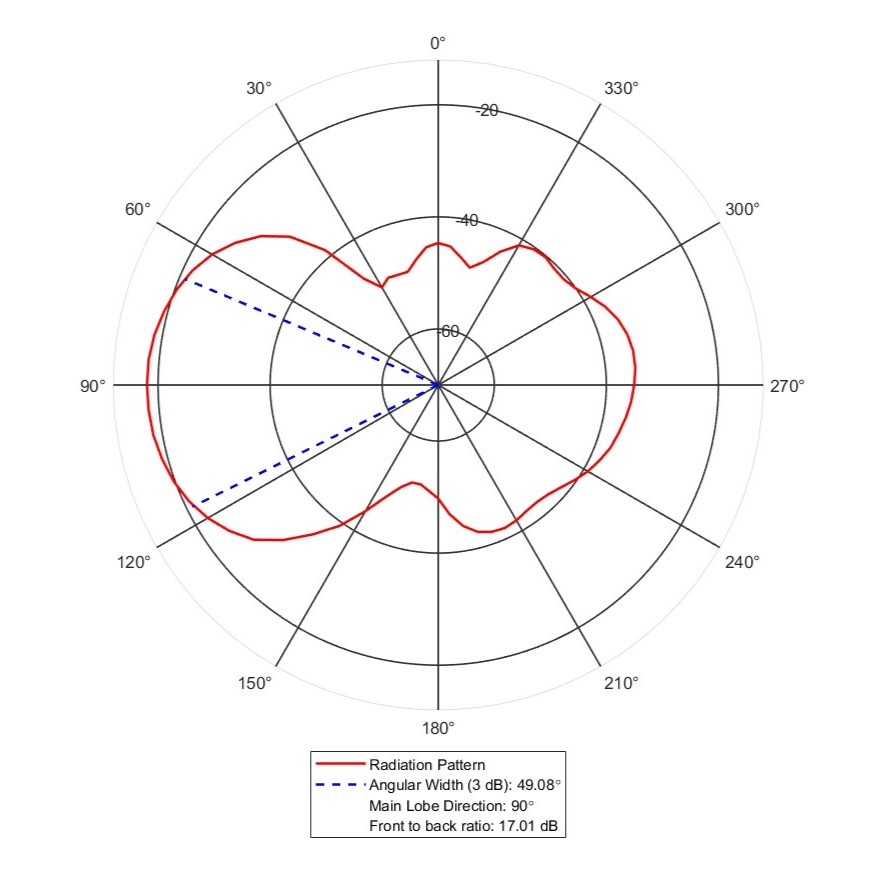
\includegraphics[width=\textwidth]{Imagens/Real_data_acquired.jpg}
         \caption{Real data acquired}
         \label{cap4:sec4:subsec1:fig1:a}
     \end{subfigure}
     \hspace{1mm}
     \begin{subfigure}{0.78\textwidth}
         \centering
         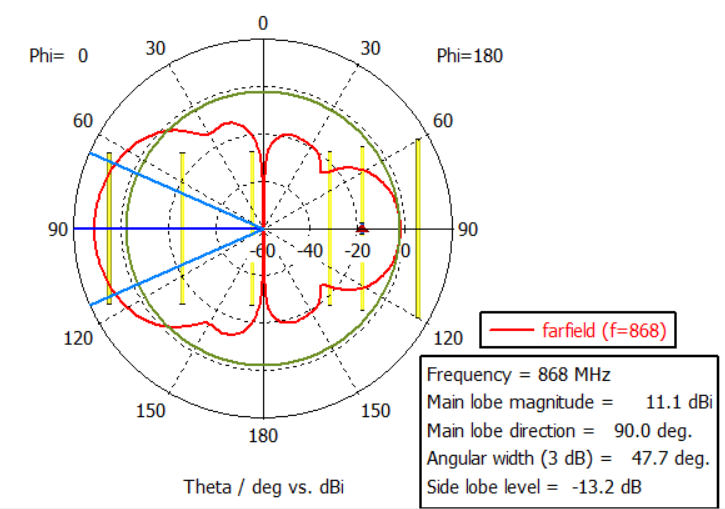
\includegraphics[width=\textwidth]{Imagens/simulationv3.png}
         \caption{Simulation of the radiation pattern}
         \label{cap4:sec4:subsec1:fig1:b}
     \end{subfigure}
        \caption{Comparison of real and simulated radiation pattern.}
        \label{cap4:sec4:subsec1:fig1}
\end{figure}

%-----------------------------------------------------------------------------------------------------
\subsection{Antenna with Band-Pass Filter}
%-----------------------------------------------------------------------------------------------------

The inclusion of the band-pass filter introduces a small insertion loss and minor modifications to the radiation pattern, which are visible when comparing the measurement to the simulation, as illustrated in Figure \ref{cap4:sec4:subsec2:fig1}

\begin{figure}[H]
     \centering
     \begin{subfigure}{0.45\textwidth}
         \centering
         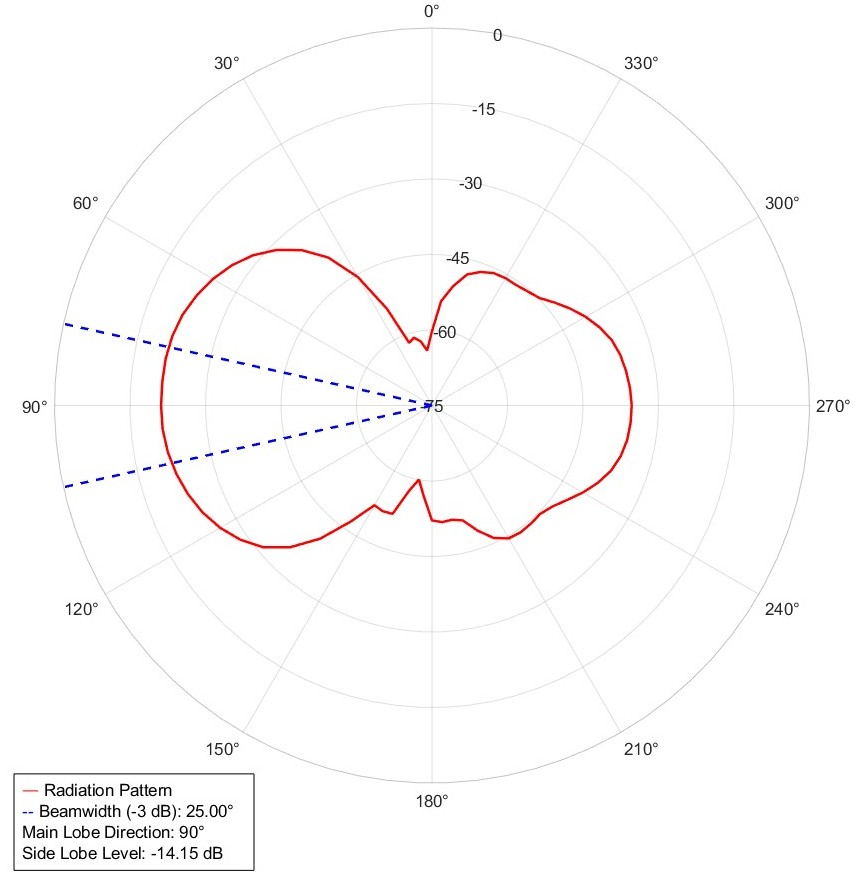
\includegraphics[width=\textwidth]{Imagens/Real_data_with_filter.jpg}
         \caption{Real data acquired with 868 MHz band-pass filter}
         \label{cap4:sec4:subsec2:fig1:a}
     \end{subfigure}
     \hspace{1mm}
     \begin{subfigure}{0.69\textwidth}
         \centering
         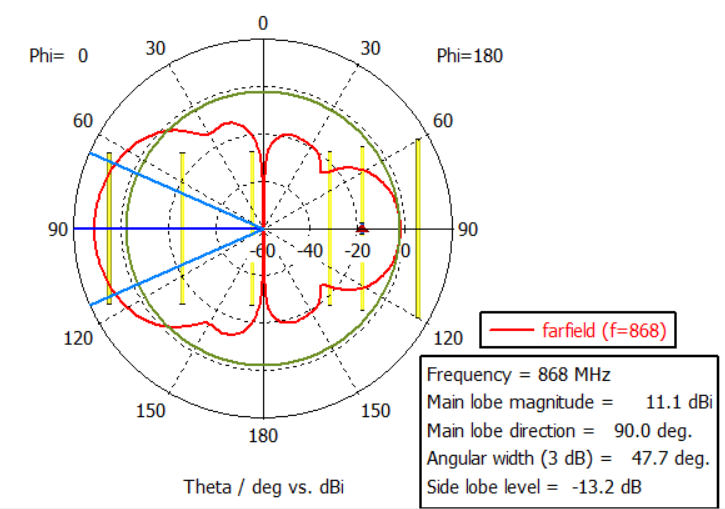
\includegraphics[width=\textwidth]{Imagens/simulationv3.png}
         \caption{Simulation of the radiation pattern on CST Studio Suite}
         \label{cap4:sec4:subsec2:fig1:b}
     \end{subfigure}
        \caption{Comparison of real and simulated radiation pattern. Antenna with band-pass filter.}
        \label{cap4:sec4:subsec2:fig1}
\end{figure}


%-----------------------------------------------------------------------------------------------------
\subsection{Antenna with Band-Pass Filter and Balun}
%-----------------------------------------------------------------------------------------------------

Adding the balun modifies the current distribution in the antenna, slightly affecting the shape of the radiation pattern compared to the previous configuration, as it is possible to visualise in Figure~\ref{cap4:sec4:subsec3:fig1}.

\begin{figure}[H]
     \centering
     \begin{subfigure}{0.45\textwidth}
         \centering
         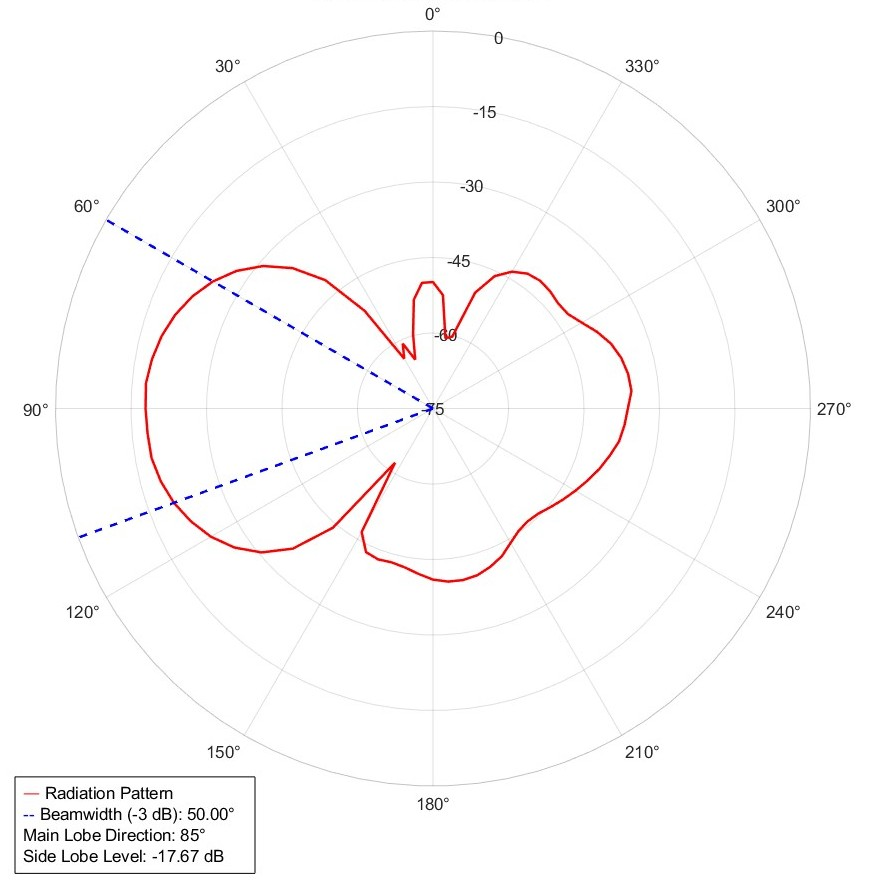
\includegraphics[width=\textwidth]{Imagens/media_real.jpg}
         \caption{Real data acquired with 868 MHz band-pass filter and balun.}
         \label{cap4:sec4:subsec3:fig1:a}
     \end{subfigure}
     \hspace{1mm}
     \begin{subfigure}{0.69\textwidth}
         \centering
         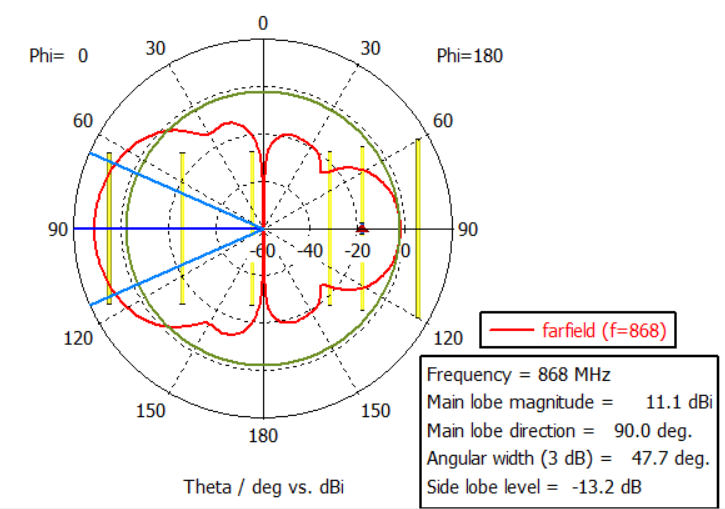
\includegraphics[width=\textwidth]{Imagens/simulationv3.png}
         \caption{Simulation of the radiation pattern on CST Studio Suite}
         \label{cap4:sec4:subsec3:fig1:b}
     \end{subfigure}
        \caption{Comparison of real and simulated radiation pattern. Antenna with band-pass filter and balun.}
        \label{cap4:sec4:subsec3:fig1}
\end{figure}

The inclusion of the band-pass filter introduces a small insertion loss ($\approx$ 3 dB) without significantly altering the main lobe of the radiation pattern.




%-----------------------------------------------------------------------------------------------------
\subsection{Antenna with Band-Pass Filter, Balun, and Impedance Matching Network}
%-----------------------------------------------------------------------------------------------------




The full configuration, including the impedance matching network, provides the most realistic representation of the final system, as can be seen in Figure \ref{cap4:sec4:subsec4:fig1}. Interestingly, the inclusion of the additional components not only preserved the main radiation characteristics but also brought the measured pattern into closer agreement with the theoretical model, showed in Figure \ref{cap4:sec4:subsec4:fig2}. Minor deviations remain, primarily due to practical insertion losses and environmental reflections.

\begin{figure}[H]
    \centering
    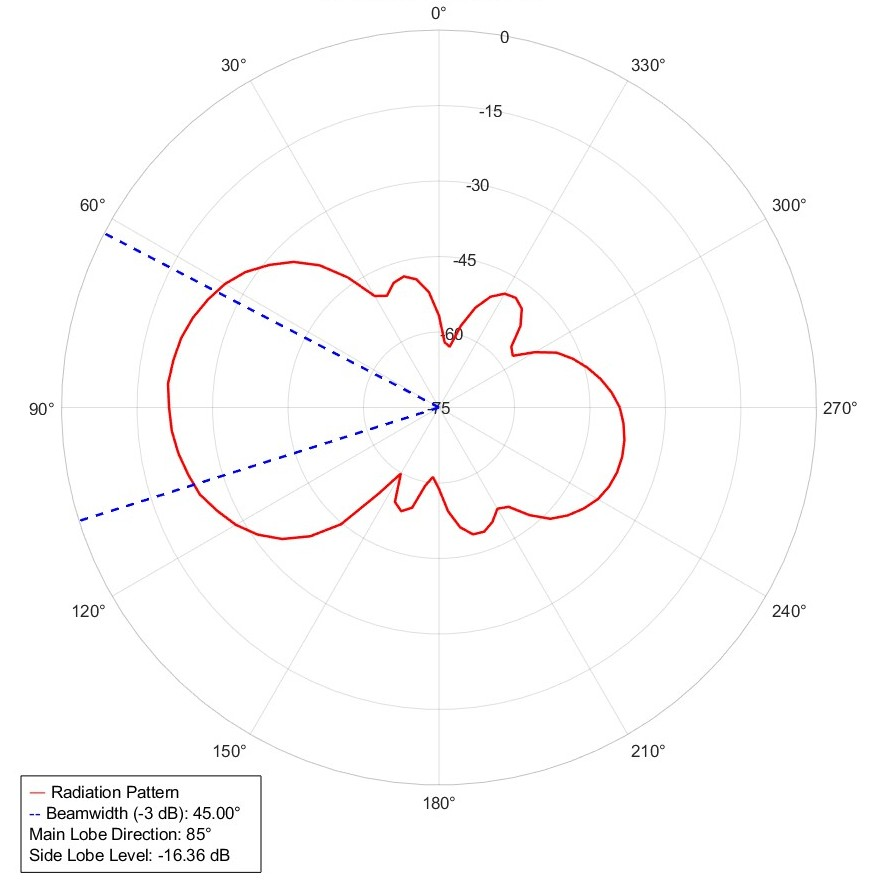
\includegraphics[width=0.65\textwidth]{Imagens/medianew.jpg}
    \caption{Measured data with filter, balun and impedance matching.}
    \label{cap4:sec4:subsec4:fig1}
\end{figure}

\begin{figure}[H]
    \centering
    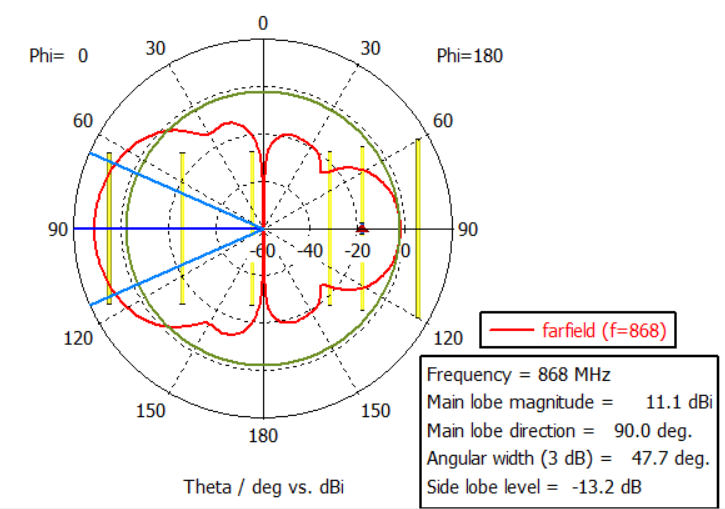
\includegraphics[width=0.95\textwidth]{Imagens/simulationv3.png}
    \caption{Simulated radiation pattern outcome from CST Studio Suite.}
    \label{cap4:sec4:subsec4:fig2}
\end{figure}


\subsubsection{3D Radiation Pattern}

Although two-dimensional radiation patterns are useful for quickly assessing antenna performance, they provide a partial view of how the radiated power is distributed in space. A full three-dimensional radiation pattern offers a more complete characterisation, allowing to see asymmetries and distortions that might not be evident in 2D slices. For this reason, a 3D measurement was carried out to complement the 2D analyses.

The three-dimensional radiation pattern of the complete antenna system was also measured and compared with the simulated model obtained in CST Studio Suite, as shown in Figure \ref{cap4:sec4:subsec4:fig3} and Figure \ref{cap4:sec4:subsec4:fig4}. Despite some distortions observed in the experimental result, a general agreement with the simulation can be identified. This confirms that the proposed measurement system is able to operate with two degrees of freedom and to characterise the radiation pattern in three dimensions.

\begin{figure}[H]
    \centering
    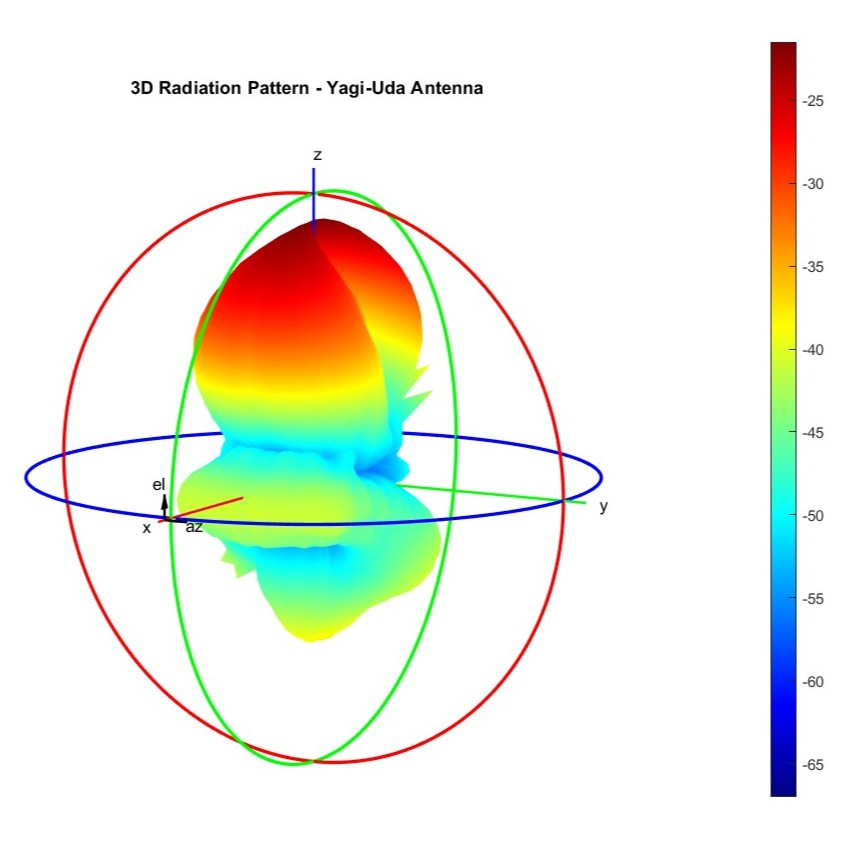
\includegraphics[width=0.7\textwidth]{Imagens/new_3d.jpg}
    \caption{Measured 3D radiation pattern.}
    \label{cap4:sec4:subsec4:fig3}
\end{figure}

\begin{figure}[H]
    \centering
    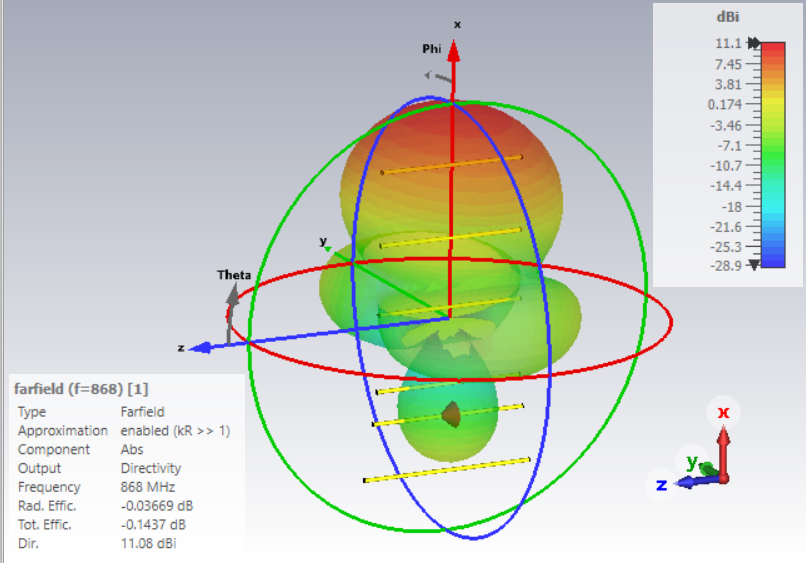
\includegraphics[width=0.7\textwidth]{Imagens/3Dsimulation.png}
    \caption{Simulated 3D radiation pattern from CST Studio Suite.}
    \label{cap4:sec4:subsec4:fig4}
\end{figure}


%-----------------------------------------------------------------------------------------------------
\section{Discussion of Results}
%-----------------------------------------------------------------------------------------------------

This section will be developed to provide both a concise overview of the obtained measurements and a summary of the main observations. The individual characterisation of each system component, such as the antenna, band-pass filter, balun, and impedance matching network, offers insight into performance and potential influence of each element on the overall system behaviour. The antenna designed and built provided good matching and radiation characteristics near the intended ISM frequency of 868~MHz, when compared with theoretical results. The band-pass filter introduced the expected insertion loss but providing frequency selectivity. The balun showed low differential-mode loss and high common-mode suppression, while the impedance matching network further optimised power transfer to the measurement system.\\
\vspace{-0.1em}
\indent It is worth noticing that the antenna gain could be indirectly estimated using the measured received power with the AD8313 RF module, the Friis equation (\ref{eq:friis}), and the previously characterised $S_{11}$ and VSWR. The estimated gain, considering the Yagi–Uda antenna’s approximate 10~dB rating, aligns well with the calculated results. This agreement provides additional validation of the antenna performance and overall system design.\\
\vspace{-0.1em}
\indent Radiation pattern measurements were performed incrementally, starting with the antenna alone and adding the filter, balun, and impedance matching network. The main lobe direction and beamwidth were generally consistent with the simulations, while minor deviations were observed as additional components were introduced. Power levels also varied with the inclusion of each component, as expected from insertion loss and other practical effects.\\
\vspace{-0.1em}
\indent In addition to the azimuthal radiation patterns, the three-dimensional radiation pattern of the complete antenna system was obtained and compared with the simulated outcome. The experimental measurement showed discrepancies with respect to the simulated model, particularly in secondary lobes, which can be attributed to environmental factors and the presence of additional circuit components, such as the balun and the impedance matching network, that were not considered in the CST simulation. Nevertheless, the main lobe of the measured pattern resembles that of the simulation, highlighting the directional characteristics expected from a Yagi–Uda antenna and allowing the identification of secondary lobes.\\
\vspace{-0.1em}
\indent Overall, the collected data provide a comprehensive record of the experimental behaviour of the system components and their interactions. The following chapter highlights the results, outlining their implications and guiding conclusions for the final system design.
